% Contextos de ejecución del firmware en el ESP32 (Tarea 2, preguntas 3 y 4).
\documentclass[border=4pt]{standalone}
% Estilo común de los diagramas: imita el tema por defecto de Mermaid usado en
% proyecto_1_grupal/docs/avance2/diagramas (nodos lavanda, grupos amarillos,
% etiquetas de flecha sobre gris, líneas punteadas para lo no permanente).
\usepackage[T1]{fontenc}
\usepackage[utf8]{inputenc}
\usepackage[scaled=0.95]{helvet}
\renewcommand{\familydefault}{\sfdefault}
\usepackage{amsmath}
\usepackage{tikz}
\usetikzlibrary{arrows.meta,positioning,fit,backgrounds,calc}
\definecolor{nodofondo}{HTML}{ECECFF}
\definecolor{nodoborde}{HTML}{9370DB}
\definecolor{grupofondo}{HTML}{FFFFDE}
\definecolor{grupoborde}{HTML}{AAAA33}
\definecolor{etiqueta}{HTML}{E8E8E8}
\definecolor{linea}{HTML}{333333}
\tikzset{
  every node/.style={text=linea},
  nodo/.style={draw=nodoborde, fill=nodofondo, line width=0.6pt, align=center,
    inner xsep=9pt, inner ysep=7pt, minimum height=13mm, font=\small},
  opcional/.style={nodo, dash pattern=on 4pt off 3pt, fill=black!3},
  flecha/.style={draw=linea, line width=0.6pt, -{Triangle[length=2.2mm,width=2mm]}},
  punteada/.style={flecha, dash pattern=on 4pt off 3pt},
  lbl/.style={fill=etiqueta, inner sep=2pt, align=center, font=\small},
  grupo/.style={draw=grupoborde, fill=grupofondo, line width=0.6pt, inner sep=7mm},
  titulo/.style={font=\small, anchor=north, inner sep=3pt},
}

\begin{document}
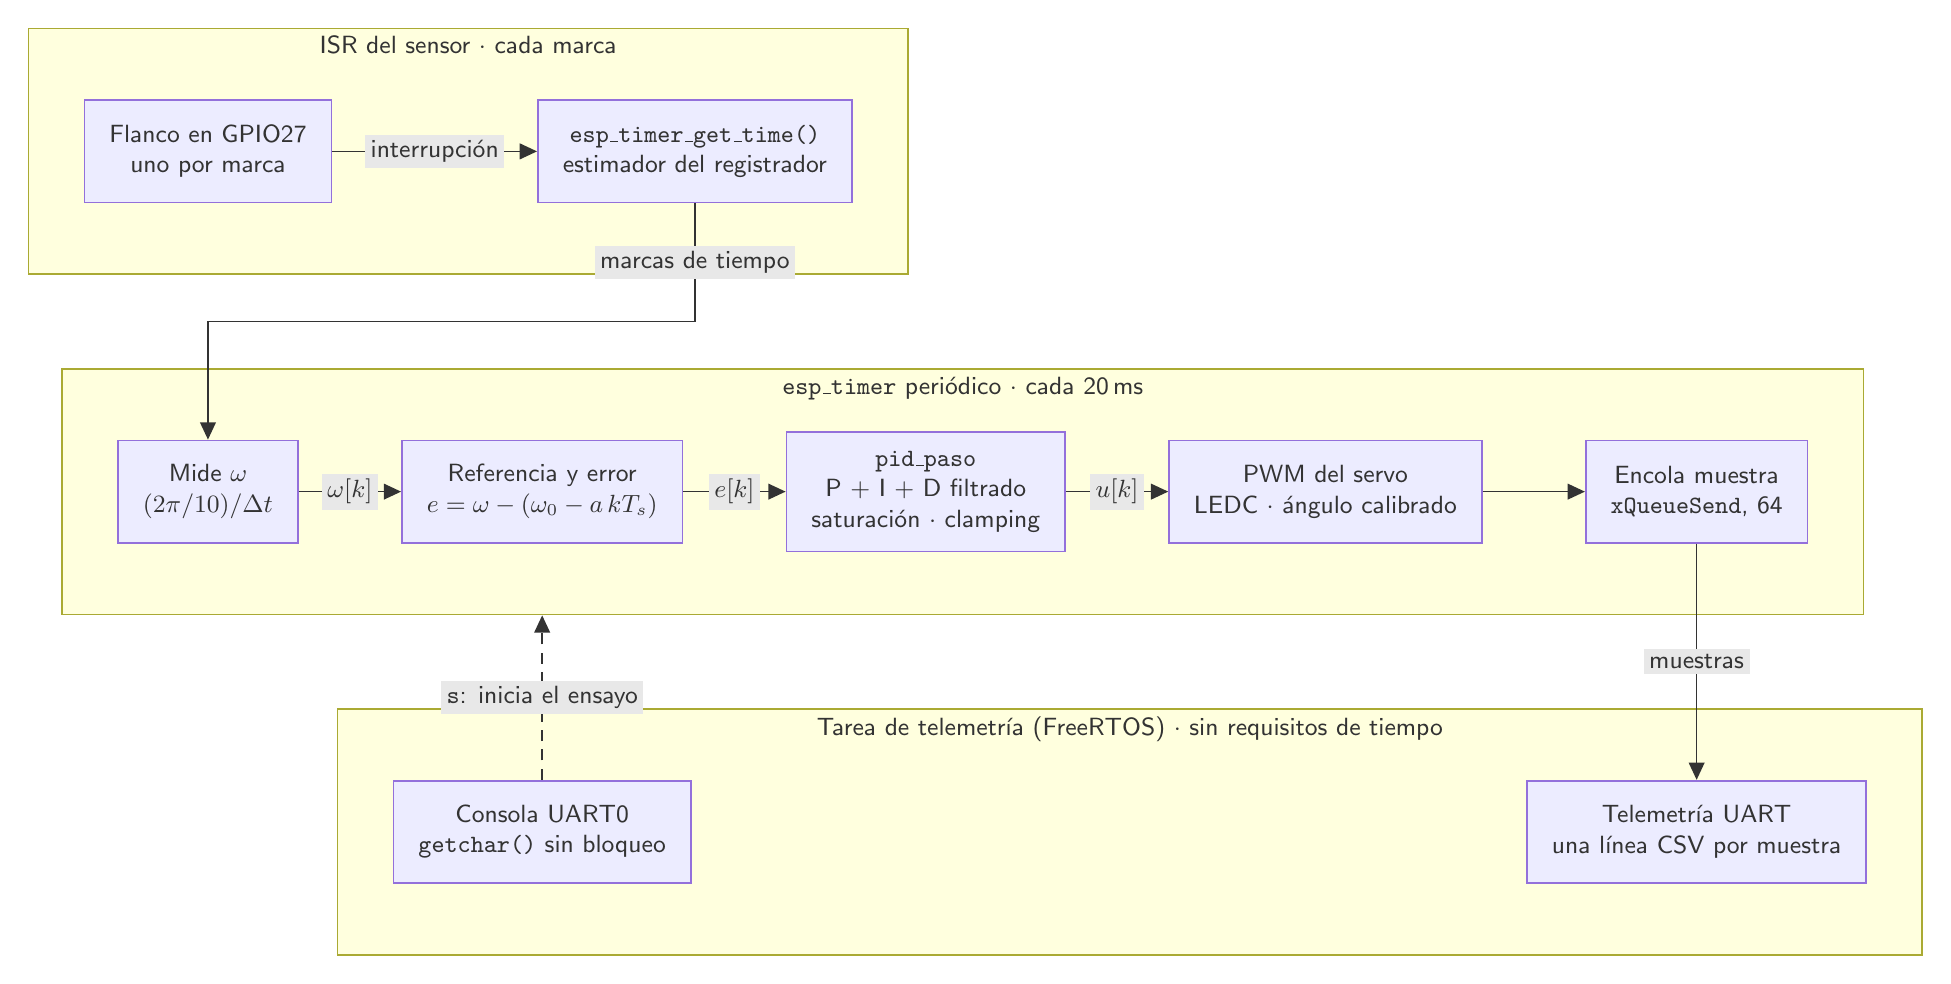
\begin{tikzpicture}
  % ISR del encoder
  \node[nodo] (fl) {Flanco en GPIO27\\uno por marca};
  \node[nodo, right=26mm of fl] (st) {\texttt{esp\_timer\_get\_time()}\\estimador del registrador};

  % Temporizador periódico
  \node[nodo, below=30mm of fl] (med) {Mide $\omega$\\$(2\pi/10)/\Delta t$};
  \node[nodo, right=13mm of med] (refk) {Referencia y error\\$e=\omega-(\omega_0-a\,kT_s)$};
  \node[nodo, right=13mm of refk] (pidk) {\texttt{pid\_paso}\\P + I + D filtrado\\saturación $\cdot$ clamping};
  \node[nodo, right=13mm of pidk] (pwmk) {PWM del servo\\LEDC $\cdot$ ángulo calibrado};
  \node[nodo, right=13mm of pwmk] (col) {Encola muestra\\\texttt{xQueueSend}, 64};

  % Bucle principal
  \node[nodo, below=30mm of refk] (con) {Consola UART0\\\texttt{getchar()} sin bloqueo};
  \node[nodo] (tel) at (con -| col) {Telemetría UART\\una línea CSV por muestra};

  \begin{scope}[on background layer]
    \node[grupo, fit=(fl)(st), inner ysep=9mm] (ga) {};
    \node[titulo] at (ga.north) {ISR del sensor $\cdot$ cada marca};
    \node[grupo, fit=(med)(col), inner ysep=9mm] (gb) {};
    \node[titulo] at (gb.north) {\texttt{esp\_timer} periódico $\cdot$ cada 20\,ms};
    \node[grupo, fit=(con)(tel), inner ysep=9mm] (gc) {};
    \node[titulo] at (gc.north) {Tarea de telemetría (FreeRTOS) $\cdot$ sin requisitos de tiempo};
  \end{scope}

  \draw[flecha] (fl) -- node[lbl]{interrupción} (st);
  \draw[flecha] (med) -- node[lbl]{$\omega[k]$} (refk);
  \draw[flecha] (refk) -- node[lbl]{$e[k]$} (pidk);
  \draw[flecha] (pidk) -- node[lbl]{$u[k]$} (pwmk);
  \draw[flecha] (pwmk) -- (col);
  \coordinate (medio) at ($(ga.south)!0.5!(gb.north)$);
  \draw[flecha] (st.south) -- node[lbl]{marcas de tiempo} (st.south |- medio) -| (med.north);
  \draw[flecha] (col.south) -- node[lbl]{muestras} (tel.north);
  \draw[punteada] (con.north) -- node[lbl]{\texttt{s}: inicia el ensayo} (con.north |- gb.south);
\end{tikzpicture}
\end{document}
